\section{Distribution of packet loss over distance}
\begin{frame}{Packet loss}{Expectations}
    \begin{block}{Signal and noise models}
    \begin{itemize}
		\item Attenuation caused by the air is minimum
		\item Possible Dirichlet boundaries: the water is 0..100\% reflective
		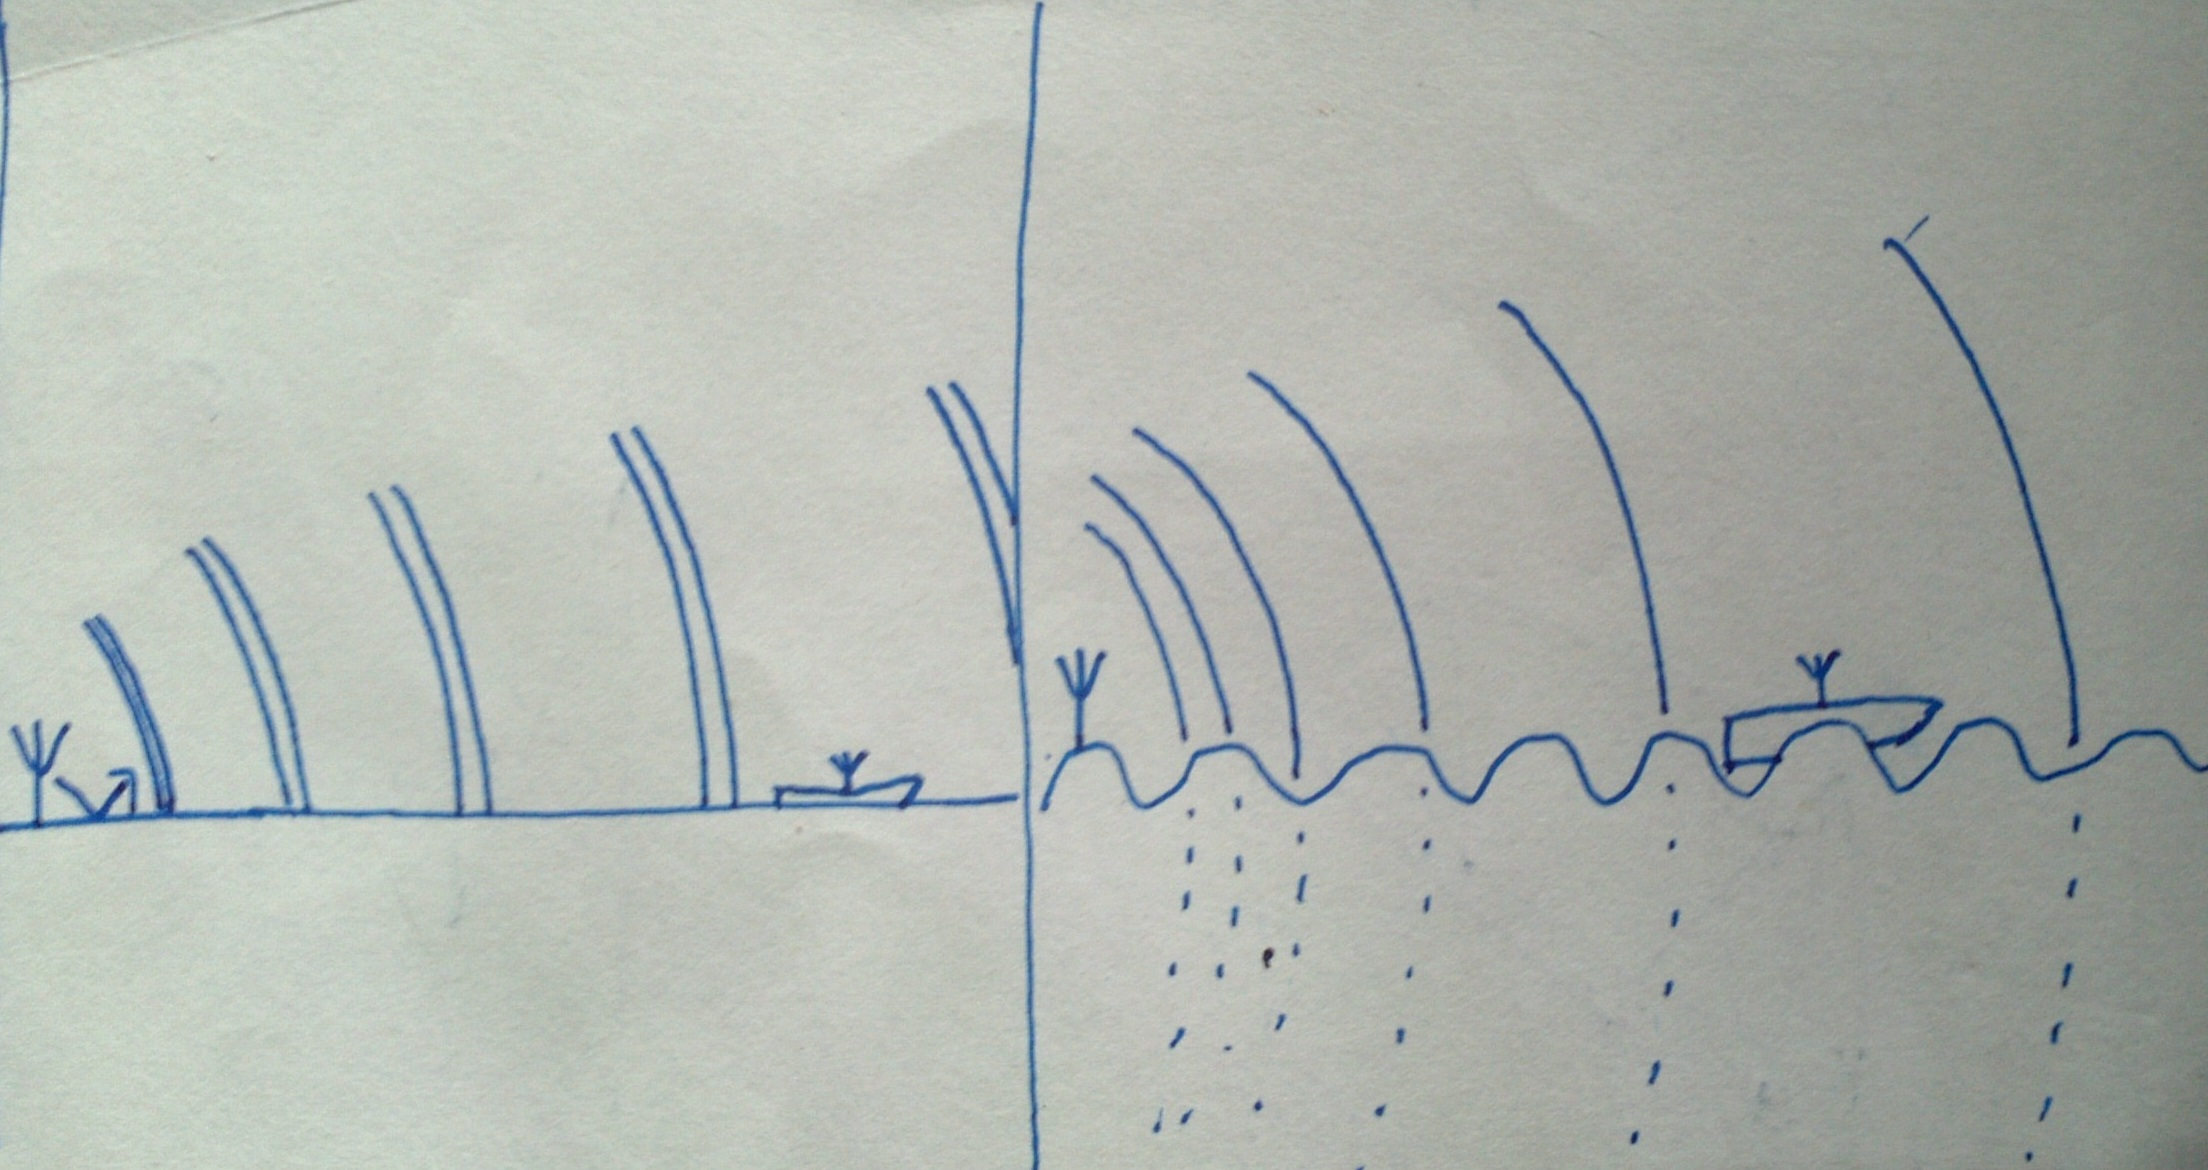
\includegraphics[width=8.4cm]{img/propagation}
		\item In still weather on the open water the expected results are better
    \end{itemize}
    \end{block}
\end{frame}
\begin{frame}{Packet loss}{Simulation}
    \begin{block}{Monte-Carlo simulation of expected Packet-loss}
    \includegraphics[trim = 0mm 80mm 0mm 80mm, clip, width=\textwidth]{img/packetloss}
    \end{block}
\end{frame}

\begin{frame}{Packet loss}{Measurement}
    \begin{block}{Measurement setup}
		\item Optimal work-time and high resolution:
		\item Gaussian distribution of measurement points
		
    \end{block}
\end{frame}
